%% Beginning of file 'sample631.tex'
%%
%% Modified 2022 May  
%%
%% This is a sample manuscript marked up using the
%% AASTeX v6.31 LaTeX 2e macros.
%%
%% AASTeX is now based on Alexey Vikhlinin's emulateapj.cls 
%% (Copyright 2000-2015).  See the classfile for details.

%% AASTeX requires revtex4-1.cls and other external packages such as
%% latexsym, graphicx, amssymb, longtable, and epsf.  Note that as of 
%% Oct 2020, APS now uses revtex4.2e for its journals but remember that 
%% AASTeX v6+ still uses v4.1. All of these external packages should 
%% already be present in the modern TeX distributions but not always.
%% For example, revtex4.1 seems to be missing in the linux version of
%% TexLive 2020. One should be able to get all packages from www.ctan.org.
%% In particular, revtex v4.1 can be found at 
%% https://www.ctan.org/pkg/revtex4-1.

%% The first piece of markup in an AASTeX v6.x document is the \documentclass
%% command. LaTeX will ignore any data that comes before this command. The 
%% documentclass can take an optional argument to modify the output style.
%% The command below calls the preprint style which will produce a tightly 
%% typeset, one-column, single-spaced document.  It is the default and thus
%% does not need to be explicitly stated.
%%
%% using aastex version 6.3
\documentclass[twocolumn,times]{aastex631}

%% The default is a single spaced, 10 point font, single spaced article.
%% There are 5 other style options available via an optional argument. They
%% can be invoked like this:
%%
%% \documentclass[arguments]{aastex631}
%% 
%% where the layout options are:
%%
%%  twocolumn   : two text columns, 10 point font, single spaced article.
%%                This is the most compact and represent the final published
%%                derived PDF copy of the accepted manuscript from the publisher
%%  manuscript  : one text column, 12 point font, double spaced article.
%%  preprint    : one text column, 12 point font, single spaced article.  
%%  preprint2   : two text columns, 12 point font, single spaced article.
%%  modern      : a stylish, single text column, 12 point font, article with
%% 		  wider left and right margins. This uses the Daniel
%% 		  Foreman-Mackey and David Hogg design.
%%  RNAAS       : Supresses an abstract. Originally for RNAAS manuscripts 
%%                but now that abstracts are required this is obsolete for
%%                AAS Journals. Authors might need it for other reasons. DO NOT
%%                use \begin{abstract} and \end{abstract} with this style.
%%
%% Note that you can submit to the AAS Journals in any of these 6 styles.
%%
%% There are other optional arguments one can invoke to allow other stylistic
%% actions. The available options are:
%%
%%   astrosymb    : Loads Astrosymb font and define \astrocommands. 
%%   tighten      : Makes baselineskip slightly smaller, only works with 
%%                  the twocolumn substyle.
%%   times        : uses times font instead of the default
%%   linenumbers  : turn on lineno package.
%%   trackchanges : required to see the revision mark up and print its output
%%   longauthor   : Do not use the more compressed footnote style (default) for 
%%                  the author/collaboration/affiliations. Instead print all
%%                  affiliation information after each name. Creates a much 
%%                  longer author list but may be desirable for short 
%%                  author papers.
%% twocolappendix : make 2 column appendix.
%%   anonymous    : Do not show the authors, affiliations and acknowledgments 
%%                  for dual anonymous review.
%%
%% these can be used in any combination, e.g.
%%
%% \documentclass[twocolumn,linenumbers,trackchanges]{aastex631}
%%
%% AASTeX v6.* now includes \hyperref support. While we have built in specific
%% defaults into the classfile you can manually override them with the
%% \hypersetup command. For example,
%%
%% \hypersetup{linkcolor=red,citecolor=green,filecolor=cyan,urlcolor=magenta}
%%
%% will change the color of the internal links to red, the links to the
%% bibliography to green, the file links to cyan, and the external links to
%% magenta. Additional information on \hyperref options can be found here:
%% https://www.tug.org/applications/hyperref/manual.html#x1-40003
%%
%% Note that in v6.3 "bookmarks" has been changed to "true" in hyperref
%% to improve the accessibility of the compiled pdf file.
%%
%% If you want to create your own macros, you can do so
%% using \newcommand. Your macros should appear before
%% the \begin{document} command.
%%
\newcommand{\vdag}{(v)^\dagger}
\newcommand\aastex{AAS\TeX}
\newcommand\latex{La\TeX}
\defcitealias{1991MNRAS.251..545H}{H91}
\usepackage{comment}

%% Reintroduced the \received and \accepted commands from AASTeX v5.2
\received{\today}
\revised{XXX}
\accepted{YYY}

%% Command to document which AAS Journal the manuscript was submitted to.
%% Adds "Submitted to " the argument.
%\submitjournal{AJ}

%% For manuscript that include authors in collaborations, AASTeX v6.31
%% builds on the \collaboration command to allow greater freedom to 
%% keep the traditional author+affiliation information but only show
%% subsets. The \collaboration command now must appear AFTER the group
%% of authors in the collaboration and it takes TWO arguments. The last
%% is still the collaboration identifier. The text given in this
%% argument is what will be shown in the manuscript. The first argument
%% is the number of author above the \collaboration command to show with
%% the collaboration text. If there are authors that are not part of any
%% collaboration the \nocollaboration command is used. This command takes
%% one argument which is also the number of authors above to show. A
%% dashed line is shown to indicate no collaboration. This example manuscript
%% shows how these commands work to display specific set of authors 
%% on the front page.
%%
%% For manuscript without any need to use \collaboration the 
%% \AuthorCollaborationLimit command from v6.2 can still be used to 
%% show a subset of authors.
%
%\AuthorCollaborationLimit=2
%
%% will only show Schwarz & Muench on the front page of the manuscript
%% (assuming the \collaboration and \nocollaboration commands are
%% commented out).
%%
%% Note that all of the author will be shown in the published article.
%% This feature is meant to be used prior to acceptance to make the
%% front end of a long author article more manageable. Please do not use
%% this functionality for manuscripts with less than 20 authors. Conversely,
%% please do use this when the number of authors exceeds 40.
%%
%% Use \allauthors at the manuscript end to show the full author list.
%% This command should only be used with \AuthorCollaborationLimit is used.

%% The following command can be used to set the latex table counters.  It
%% is needed in this document because it uses a mix of latex tabular and
%% AASTeX deluxetables.  In general it should not be needed.
%\setcounter{table}{1}

%%%%%%%%%%%%%%%%%%%%%%%%%%%%%%%%%%%%%%%%%%%%%%%%%%%%%%%%%%%%%%%%%%%%%%%%%%%%%%%%
%%
%% The following section outlines numerous optional output that
%% can be displayed in the front matter or as running meta-data.
%%
%% If you wish, you may supply running head information, although
%% this information may be modified by the editorial offices.
\shorttitle{On the Red Clump Age Method}
\shortauthors{Chriss and Worthey}
%%
%% You can add a light gray and diagonal water-mark to the first page 
%% with this command:
%% \watermark{text}
%% where "text", e.g. DRAFT, is the text to appear.  If the text is 
%% long you can control the water-mark size with:
%% \setwatermarkfontsize{dimension}
%% where dimension is any recognized LaTeX dimension, e.g. pt, in, etc.
%%
%%%%%%%%%%%%%%%%%%%%%%%%%%%%%%%%%%%%%%%%%%%%%%%%%%%%%%%%%%%%%%%%%%%%%%%%%%%%%%%%
%\graphicspath{{./}{figures/}}
%% This is the end of the preamble.  Indicate the beginning of the
%% manuscript itself with \begin{document}.

\begin{document}

\title{On the Age Calibration of Open Clusters using Red Clump Stars}

%% LaTeX will automatically break titles if they run longer than
%% one line. However, you may use \\ to force a line break if
%% you desire. In v6.31 you can include a footnote in the title.

%% A significant change from earlier AASTEX versions is in the structure for 
%% calling author and affiliations. The change was necessary to implement 
%% auto-indexing of affiliations which prior was a manual process that could 
%% easily be tedious in large author manuscripts.
%%
%% The \author command is the same as before except it now takes an optional
%% argument which is the 16 digit ORCID. The syntax is:
%% \author[xxxx-xxxx-xxxx-xxxx]{Author Name}
%%
%% This will hyperlink the author name to the author's ORCID page. Note that
%% during compilation, LaTeX will do some limited checking of the format of
%% the ID to make sure it is valid. If the "orcid-ID.png" image file is 
%% present or in the LaTeX pathway, the OrcID icon will appear next to
%% the authors name.
%%
%% Use \affiliation for affiliation information. The old \affil is now aliased
%% to \affiliation. AASTeX v6.31 will automatically index these in the header.
%% When a duplicate is found its index will be the same as its previous entry.
%%
%% Note that \altaffilmark and \altaffiltext have been removed and thus 
%% can not be used to document secondary affiliations. If they are used latex
%% will issue a specific error message and quit. Please use multiple 
%% \affiliation calls for to document more than one affiliation.
%%
%% The new \altaffiliation can be used to indicate some secondary information
%% such as fellowships. This command produces a non-numeric footnote that is
%% set away from the numeric \affiliation footnotes.  NOTE that if an
%% \altaffiliation command is used it must come BEFORE the \affiliation call,
%% right after the \author command, in order to place the footnotes in
%% the proper location.
%%
%% Use \email to set provide email addresses. Each \email will appear on its
%% own line so you can put multiple email address in one \email call. A new
%% \correspondingauthor command is available in V6.31 to identify the
%% corresponding author of the manuscript. It is the author's responsibility
%% to make sure this name is also in the author list.
%%
%% While authors can be grouped inside the same \author and \affiliation
%% commands it is better to have a single author for each. This allows for
%% one to exploit all the new benefits and should make book-keeping easier.
%%
%% If done correctly the peer review system will be able to
%% automatically put the author and affiliation information from the manuscript
%% and save the corresponding author the trouble of entering it by hand.

%\correspondingauthor{Guy Worthey}
%\email{gworthey@wsu.edu, achriss@bowdoin.edu}

\author[0009-0003-8929-7110]{Abigail R. Chriss}
\affiliation{Department of Physics and Astronomy, Bowdoin College, 8800 College Station, Brunswick, ME 04011-8488, USA}

\author[0000-0003-1388-5525]{Guy Worthey}
\affiliation{Department of Physics and Astronomy, Washington State University, 1245 Webster Hall, Pullman, WA 99164-2814, USA}

%% Note that the \and command from previous versions of AASTeX is now
%% depreciated in this version as it is no longer necessary. AASTeX 
%% automatically takes care of all commas and "and"s between authors names.

%% AASTeX 6.31 has the new \collaboration and \nocollaboration commands to
%% provide the collaboration status of a group of authors. These commands 
%% can be used either before or after the list of corresponding authors. The
%% argument for \collaboration is the collaboration identifier. Authors are
%% encouraged to surround collaboration identifiers with ()s. The 
%% \nocollaboration command takes no argument and exists to indicate that
%% the nearby authors are not part of surrounding collaborations.

%% Mark off the abstract in the ``abstract'' environment. 
\begin{abstract}

In this study, we extend the dust-independent \citet{1991MNRAS.251..545H} relation between cluster age and $d_{B-R}$ color difference between red giant branch (RGB) and red clump (RC) to younger cluster ages. We perform membership analysis on twenty-two open clusters using \textit{Gaia} DR3 astrometry, then compute the difference in color of red giant branch and red clump $d_{B-R}$ using \textit{Gaia} photometry. We find that the trend derived from older clusters does not extrapolate to younger ages and becomes double-valued. We confirm that $d_{B-R}$ is independent of metallicity. Current stellar evolutionary isochrones do not quantitatively reproduce the trend and furthermore predict an increased color gap with a decrease in metallicity that is not echoed in the data. Integrated light models based on current isochrones exaggerate the color change over the $-0.5 <$ [Fe/H] $< 0$ interval at the few-percent level.

\end{abstract}

%% Keywords should appear after the \end{abstract} command. 
%% The AAS Journals now uses Unified Astronomy Thesaurus concepts:
%% https://astrothesaurus.org
%% You will be asked to selected these concepts during the submission process
%% but this old "keyword" functionality is maintained in case authors want
%% to include these concepts in their preprints.
\keywords{Open star clusters (1160) --- Stellar ages (1581) --- Red giant clump (1370) --- Red giant branch (1368) --- Hertzsprung Russell diagram (725)}

%% From the front matter, we move on to the body of the paper.
%% Sections are demarcated by \section and \subsection, respectively.
%% Observe the use of the LaTeX \label
%% command after the \subsection to give a symbolic KEY to the
%% subsection for cross-referencing in a \ref command.
%% You can use LaTeX's \ref and \label commands to keep track of
%% cross-references to sections, equations, tables, and figures.
%% That way, if you change the order of any elements, LaTeX will
%% automatically renumber them.
%%
%% We recommend that authors also use the natbib \citep
%% and \citet commands to identify citations.  The citations are
%% tied to the reference list via symbolic KEYs. The KEY corresponds
%% to the KEY in the \bibitem in the reference list below. 

\section{Introduction} \label{section_intro}

Star clusters represent both a crucial testing ground for the theory of stellar evolution and markers for the chemical and dynamical history of the Milky Way and other galaxies. While massive star clusters typically host multiple stellar populations \citep{2012A&ARv..20...50G}, lower-mass open clusters are currently presumed to be simple stellar populations (SSPs) of a single age and heavy element abundance pattern. Cluster ages are often derived from the color magnitude diagram (CMD), where, especially, the luminosity of the main sequence turnoff (MSTO) provides a theoretically robust chronometer \citep{1995ApJ...444L...9C}.

Even assuming perfect comparison models, distance uncertainty and line of sight dust extinction add error to age estimates. 
\citet{1991MNRAS.251..545H}, hereafter \citetalias{1991MNRAS.251..545H}, proposed a method that bypasses both dust and distance. The color of the He-burning red clump (RC) is subtracted from the color of the H-burning red giant branch (RGB) at the same luminosity. \citetalias{1991MNRAS.251..545H} used Johnson-Cousins $B$ and $R$ filters and thus the color difference is $d_{B-R}$. Age was found to track $d_{B-R}$ for clusters older than $\sim$2 Gyr and for a variety of heavy element abundances. A bonus advantage of this method is that red clump stars are $\sim$100 times brighter than MSTO stars, and thus the method could be applied to distant clusters.

The advent of star formation history reconstruction methods, where the entire CMD is fit with a swarm of stellar evolutionary isochrones \citep{2001ApJS..136...25H,2002MNRAS.332...91D}, might explain why the \citetalias{1991MNRAS.251..545H} formula has not seen wide use \citep{2016ARA&A..54...95G}. Girardi notes, however, that the reconstructions for older ages rest upon clump and RGB lifetimes, something predicted by stellar evolutionary theory only at the 20\% level.

The purpose of the present work is to confirm and extend \citetalias{1991MNRAS.251..545H}'s result. The red clump should exist in the CMD for ages as young as $\sim$200 Myr, or MSTO masses of $\sim$5 M$_\odot$. We were curious if \citetalias{1991MNRAS.251..545H}'s result extended to younger populations. To that end, we mined \textit{Gaia} open cluster data for additional clusters with red clumps, with particular attention to clusters between 200 Myr and 2 Gyr in age.

We describe cluster membership discrimination and our derivation of isochrone-based ages in $\S$\ref{section_methods}. The \citetalias{1991MNRAS.251..545H} method is addressed in $\S$\ref{section_results}, and we discuss the result in $\S$\ref{section_discussion}.

\section{Cluster Sample and Membership Analysis} \label{section_methods}

From open cluster lists \citep{2013A&A...558A..53K,2020A&A...640A...1C} we selected clusters beyond the \citetalias{1991MNRAS.251..545H} list, initially in the age range 200 Myr to 2 Gyr. As the project developed, we added a few older clusters to test the repeatability of the \citetalias{1991MNRAS.251..545H} method. Ideal clusters lie nearby and bloom richly with stars.

For each of the 22 clusters presented in Table \ref{tab:cluster BP-RP} we performed a membership analysis before applying reddening corrections and analyzing the CMD. The probabilities of membership for stars in each cluster were estimated using position ($\alpha , \delta$), proper motion ($\mu_\alpha , \mu_\delta$), and parallax ($\pi$) from \textit{Gaia} Data Release 3 (DR3). Cluster centers, proper motion central locations, and parallaxes from Simbad served as a first guess for each cluster, though we allowed drifts from these values during the fitting process. For position and proper motion, we drew annuli around the central location and computed star density (number per square degree or number per km s$^{-1}$, respectively) as a function of annulus bin radius ($r$). We employed a least squares fitter to model functions for the total stars and the field star background. We modeled the cluster spatial profile as a Gaussian with a constant-density pedestal representing field stars (Fig. \ref{fig:pos_dist}). Based on position, for example, the cluster membership probability for each star $i$ is 

$$
P_{{\rm cluster,\ }(\alpha, \delta)}(i) = \frac{N_{\rm total}(r_i) - N_{\rm field}(r_i)}{N_{\rm total}(r_i)},
$$ where $r_i$ is the distance of a star from the cluster center, and the number of counts per square degree $N$ come from two (cluster and field) function fits to the density profile. In other words, the probability is the expected fraction of member stars as a function of distance from the cluster center.

\textcolor{green}{}
\textcolor{red}{}
\begin{table*}
	\centering
	\caption{Age (log years) and errors from \citet{2020A&A...640A...1C}, color excess from \citet{2013A&A...558A..53K} (magnitude), and color difference of red clump and red giant branch and errors (magnitude). Number of stars with probability greater than 0.8 and opening angle for cone search (degrees) are also included.}
	\label{tab:cluster BP-RP}
 \begin{tabular}{lccccccc}
		\hline
  Name & Age  & E($BP-RP$) & $d_{BP-RP}$  & N$_{80}$ & Opening angle \\
     & (log years) & (mag) & (mag) &  & (deg) \\
		\hline
           Pismis 18  & 8.76 $\pm \ 0.175$ & 0.698 & 0.055 $\pm \ 0.019$ & 321 & 0.099\\
           %NGC 2447  & 8.76 $\pm \ 0.175$ & 0.067 & 0.076 $\pm 0.005$ & 815 & 0.808\\
           NGC 1907   & 8.77 $\pm \ 0.175$ & 0.670 & 0.132 $\pm 0.040$ & 15 & 0.224\\
           NGC 2660   & 8.97 $\pm \ 0.175$ & 0.627 & 0.098 $\pm 0.008$ & 257 & 0.105\\
           Melotte 71 & 8.99 $\pm \ 0.175$ & 0.139 & 0.125 $\pm 0.023$ & 213 & 0.224\\
            King 5    & 9.01 $\pm \ 0.175$ & 0.897 & 0.087 $\pm 0.006$ & 204 & 0.272\\
            NGC 2477  & 9.05 $\pm \ 0.175$ & 0.390 & 0.169 $\pm 0.004$ & 1206 & 0.450\\
            NGC 2236  & 9.06 $\pm \ 0.175$ & 0.753 & 0.078 $\pm 0.028$ & 139 & 0.210\\
            NGC  752  & 9.07 $\pm \ 0.175$ & 0.054 & 0.079 $\pm 0.005$ & 173 & 1.938\\
            NGC 1245  & 9.08 $\pm \ 0.175$ & 0.335 & 0.103 $\pm 0.004$ & 419 & 0.326\\
            NGC 6940  & 9.13 $\pm \ 0.175$ & 0.281 & 0.045 $\pm 0.008$ & 447 & 0.100\\
            NGC 6208  & 9.15 $\pm \ 0.175$ & 0.279 & 0.087 $\pm 0.005$ & 113 & 0.486\\
            NGC 2509  & 9.18 $\pm \ 0.175$ & 0.139 & 0.081 $\pm 0.012$ & 52 & 0.179\\
            NGC 7789  & 9.19 $\pm \ 0.175$ & 0.296 & 0.124 $\pm 0.004$ & 373 & 0.422\\
            NGC 2506  & 9.22 $\pm \ 0.175$ & 0.056 & 0.084 $\pm 0.004$ & 1645 & 0.263\\
            NGC 6939  & 9.23 $\pm \ 0.175$ & 0.415 & 0.118 $\pm 0.009$ & 364 & 0.245\\
            NGC 2420  & 9.24 $\pm \ 0.175$ & 0.013 & 0.082 $\pm 0.003$ & 372 & 0.210\\
         Ruprecht 68  & 9.26 $\pm \ 0.15$ & 0.446 & 0.154 $\pm \ 0.012$ & 57 & 0.221\\
	Collinder 110 & 9.26 $\pm \ 0.15$ & 0.557 & 0.071 $\pm 0.016$ & 74 & 0.627\\
            NGC 2627  & 9.27 $\pm \ 0.15$ & 0.139 & 0.078 $\pm 0.007$ & 245 & 0.260\\
		Melotte 66 & 9.63 $\pm \ 0.15$ & 0.167 & 0.127 $\pm 0.004$ & 1203 & 0.262\\
            NGC 2682  & 9.63 $\pm \ 0.15$ & 0.067 & 0.075 $\pm 0.004$ & 832 & 0.622\\
            NGC 6791  & 9.80 $\pm \ 0.15$ & 0.157 & 0.128 $\pm 0.004$ & 3452 & 0.204\\ 
		\hline
	\end{tabular}
\end{table*}

The fit for proper motion assumed an exponential density profile for the cluster on top of a constant field density (Fig. \ref{fig:pm_dist}), the only difference being that the ``distance'' is the $\Delta\mu$ from the cluster locus. The parallax distribution was fit with two Gaussians, a broad one for the field and a narrow one for the cluster (Fig. \ref{fig:plx_dist}). Cone search opening angles (column 6 in Table \ref{tab:cluster BP-RP}) were revisited if density profiles did not clearly reach an asymptote.

\begin{figure}
	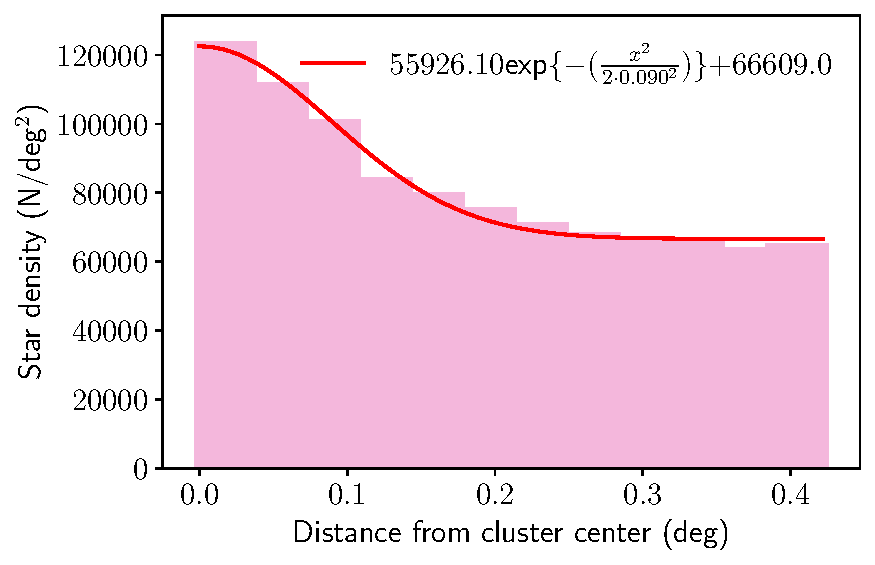
\includegraphics[width=\columnwidth]{NGC_7789_pos_dist.pdf}
    \caption{Stellar density in pragmatic units in annuli proceeding from the center of the sky position of NGC~7789. A Gaussian model is shown (red). Field star density is taken as the constant-density asymptote.}
    \label{fig:pos_dist}
\end{figure}

\begin{figure}
	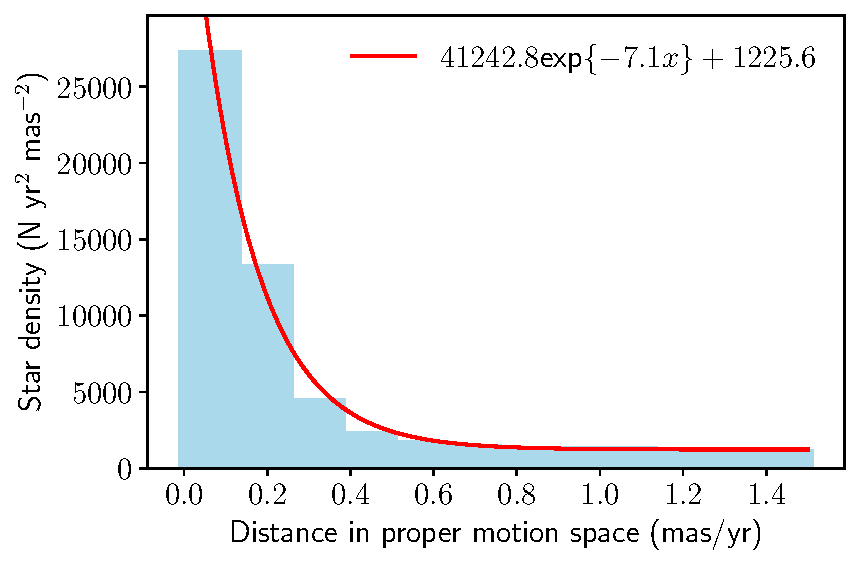
\includegraphics[width=\columnwidth]{ngc7789_pm_dist}
    \caption{Stellar density in pragmatic units in annuli proceeding from the center of the proper motion location of NGC~7789 amongst the field stars. An exponential model is shown (red). Field star density is taken as the constant-density asymptote.}
    \label{fig:pm_dist}
\end{figure}

\begin{figure}
	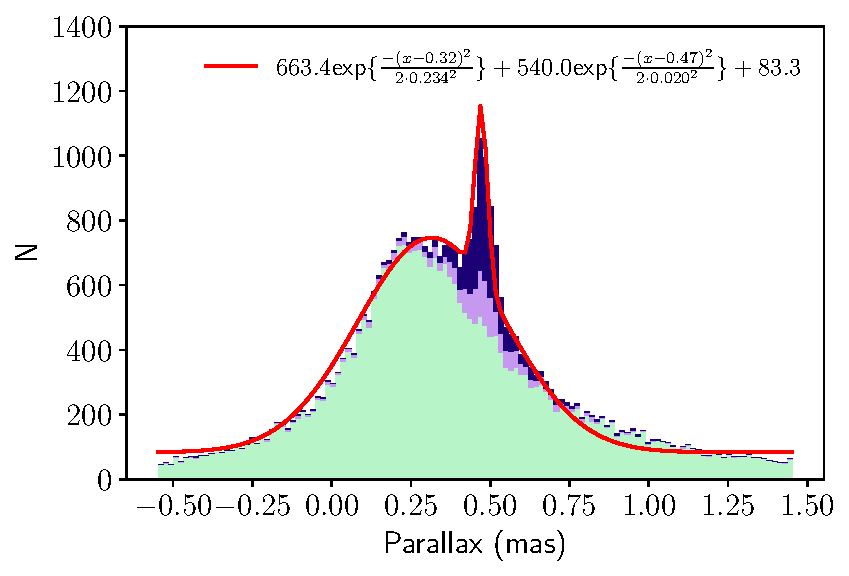
\includegraphics[width=\columnwidth]{NGC_7789_plx_dist.pdf}
    \caption{Distribution of stars in parallax in the NGC~7789 field. Stars nearest the proper motion locus (navy) and additional stars in a wider annulus (purple) form an obvious overdensity amongst the field stars (green). A two-Gaussian model is shown (red), with the broader component representing field stars.}
    \label{fig:plx_dist}
\end{figure}

Given three separate probability estimates, the combined probability from separate $P_{(\alpha, \delta)}$, $P_\mu$, and $P_\pi$ estimates is computed as in \citet{1998A&AS..133..387B}, updated to include increased dimensionality as in \citet{2022MNRAS.511.4702G}. The resultant probability distribution for NGC 7789 is shown in Fig. \ref{fig:prob_dist}.

\begin{figure}
	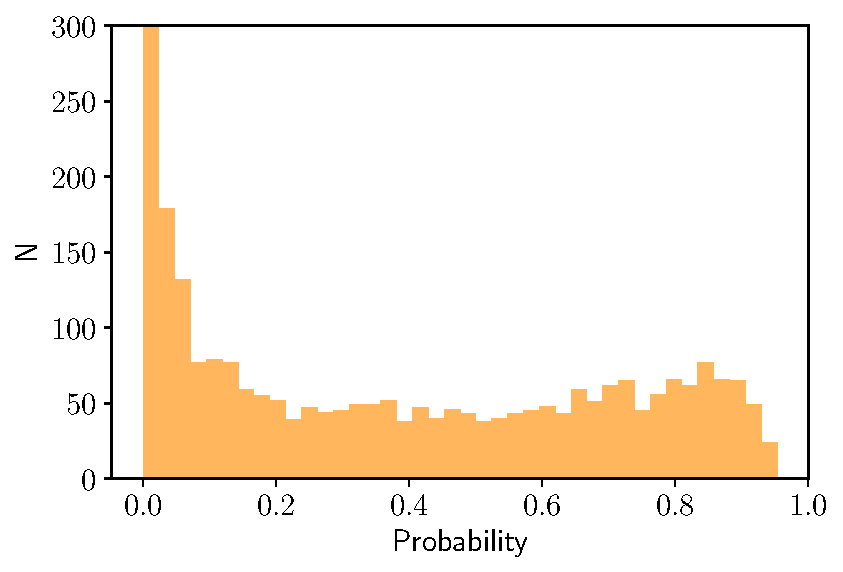
\includegraphics[width=\columnwidth]{NGC_7789_prob_dist.pdf}
    \caption{The resultant probability distribution after separate probabilities are combined for NGC~7789. The first bin contains about 20000 nonmember stars.}
    \label{fig:prob_dist}
\end{figure}

% 2.2 - Empirical calculation
\section{Results} \label{section_results}

\begin{figure}
	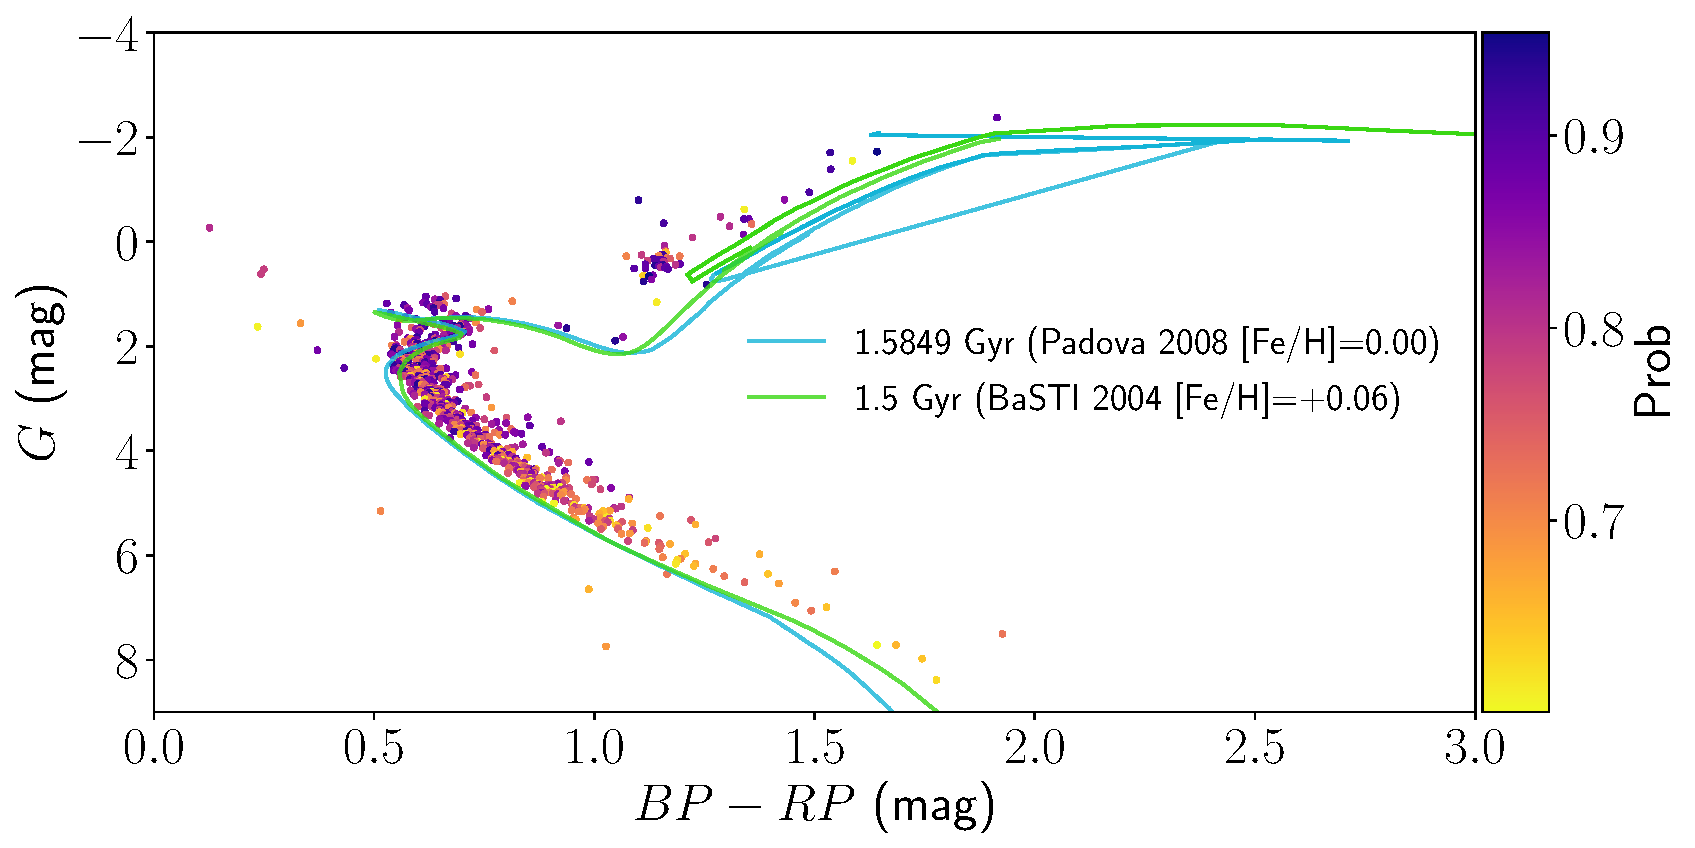
\includegraphics[width=\columnwidth]{NGC_7789_cmd.pdf}
    \caption{Color-absolute magnitude diagram in \textit{Gaia} passbands for probable members ($P > 0.7$) of NGC~7789 using the distance and reddening from Table \ref{tab:cluster BP-RP}. Symbols are color mapped by membership probability as indicated by the color bar. Example isochrones from Padova (blue, with carbon-rich stars excluded) and BaSTI (green) are shown. }
    \label{fig:cmd}
\end{figure}

From cleaned CMDs such as that of Fig. \ref{fig:cmd}, we computed clump color-magnitude location using the Tukey biweight statistic \citep{1990AJ....100...32B} in both $BP-RP$ and $G$. The error in central location was estimated as $\sigma = \sqrt{v/N}$, where $v$ is the biweight midvariance and $N$ is the number of clump stars used for the calculation. Giant branch colors at the $G$ magnitude of the red clump were found by overlaying an isochrone's RGB on the data. The synthetic RGB was then shifted left and right until 50\% of stars were bluer and 50\% of stars were redder. Once placed, the $BP-RP$ magnitude at the $G$ magnitude of the $RC$ was read from the shifted synthetic RGB. The clump stars outnumbered the RGB stars, so we expect counting statistics on the RGB to be the largest error source. We estimated RGB placement errors by shifting the theoretical RGB $\pm$ one star from the median position, and taking the average of the absolute value of those two shifts. 

We adopted ages and rough age estimate errors from \citet{2020A&A...640A...1C}, namely $\pm$ 0.175 log years for clusters younger than 9.25 log years and $\pm$ 0.15 log years for older clusters. To plot \citetalias{1991MNRAS.251..545H}'s data, we use the ages reported in the paper but scale them by 0.9 to approximately account for the drift in age scale from 1991 to now. We used the algebraic formulae in \citet{2021A&A...649A...3R} to transform from the \textit{Gaia} photometric system to Johnson-Cousins $B-R$. Color excess from \cite{2013A&A...558A..53K} was converted from E(B-V) to E($BP-RP$) using \citet{2018MNRAS.479L.102C}. 

Results are summarized in Table \ref{tab:cluster BP-RP} and shown in Fig. \ref{fig:age_calibration} with the \citetalias{1991MNRAS.251..545H} fit, transformed to logarithmic age, overlaid.

\begin{figure*}
    \centering
    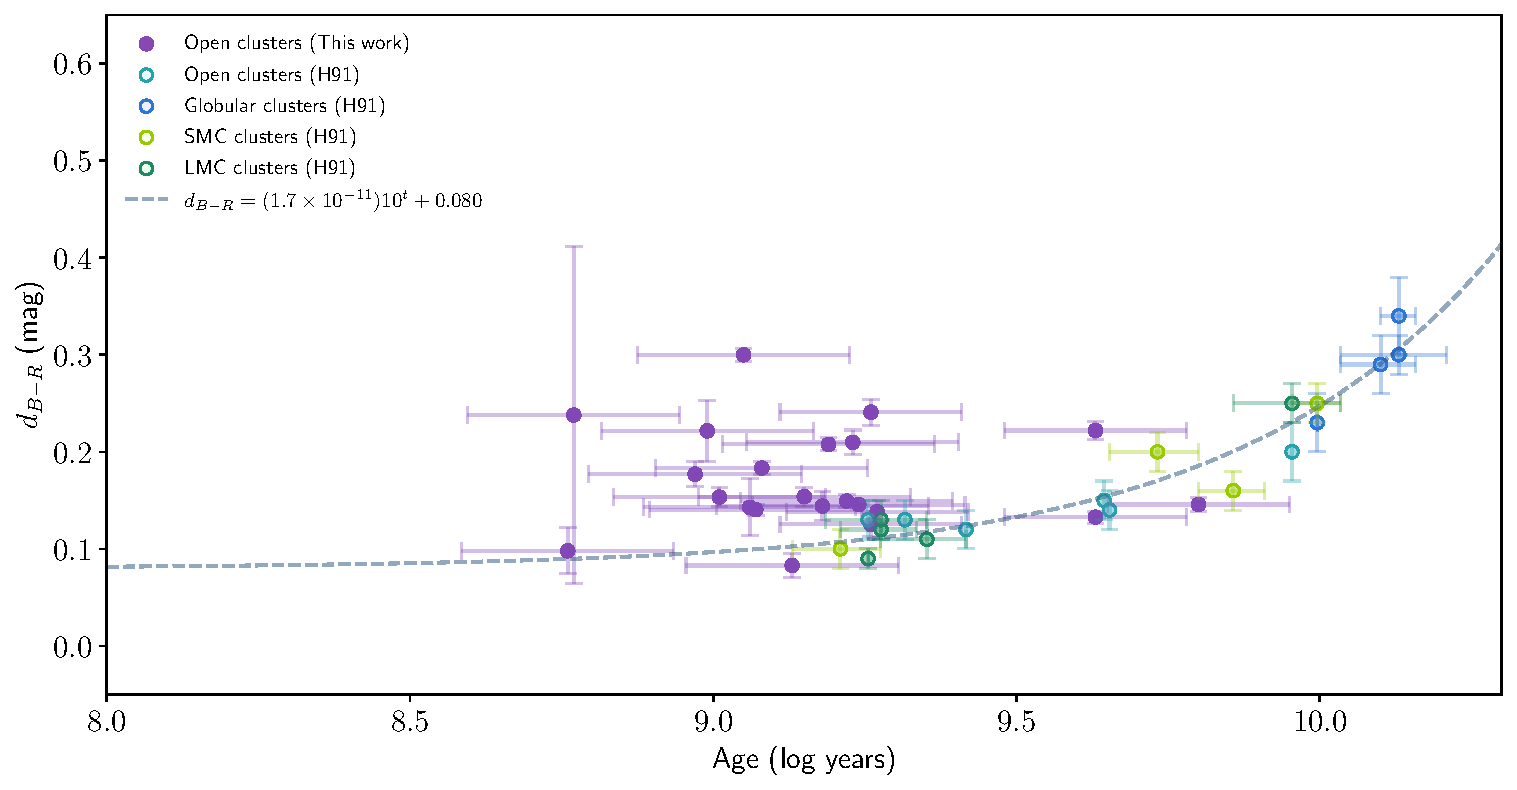
\includegraphics[width=\textwidth]{age_calibration}
    \caption{Color delta versus log age for open star clusters from this work (purple circles), along with open clusters (open blue-green circles), globular clusters (open blue circles), SMC clusters (open light green circles), and LMC clusters (open dark green circles) from \citetalias{1991MNRAS.251..545H}. The \citetalias{1991MNRAS.251..545H} linear fit (dashed line) is also shown.}
    \label{fig:age_calibration}
\end{figure*}



\section{Discussion and Conclusion} \label{section_discussion}

From Fig. \ref{fig:age_calibration} we find that the \citetalias{1991MNRAS.251..545H} line extrapolates poorly at the young end, and that many clusters have a larger clump-RGB color separation than the relation would predict. At log(age) = 9.25, or age = 1.8 Gyr, the samples overlap in age, but every cluster in the new sample shows a wider $d_{B-R}$ color separation. The magnitude of the effect exceeds any possible random or systematic uncertainties.

Even restricted to the new measurements, and further restricted to log age $< 9.5$, the scatter appears to be astrophysical. A Kolmogorov-Smirnov test on our $d_{BP-RP}$ values for clusters in our sample younger than 9.5 log years returned $p \approx 1.62 \times 10^{-5}$, indicating that the scatter is not drawn from a normal distribution. The cause of the scatter cannot be age, or we would see a slope in Fig. \ref{fig:age_calibration}. We sample metallicity span less well, but within that caveat, no metallicity dependence is evident. If neither age nor metallicity is the cause of the modulation in $d_{B-R}$, we are driven to consider more subtle causes such as variation in helium abundance, variation in the [$\alpha$/Fe] ratio, or variation in binary separation  distributions. The investigation into the cause of the scatter must await future work.

\begin{figure*}
    \centering
    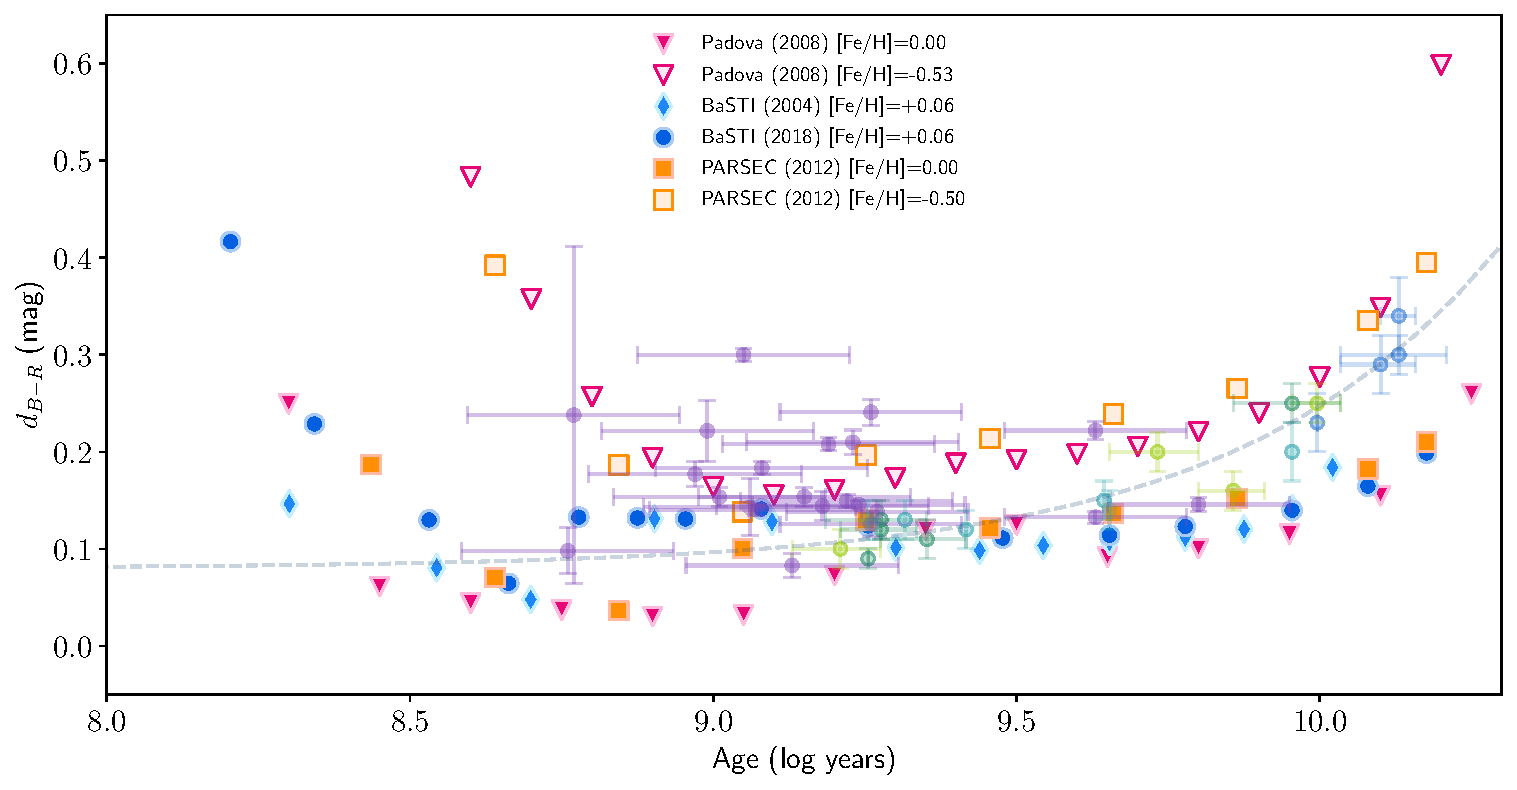
\includegraphics[width=\textwidth]{theory_age_calibration.pdf}
    \caption{Color delta versus log age. Symbols are the same as Fig. \ref{fig:age_calibration} with the addition of predictions from various isochrone sets: We show \citep{2008A&A...482..883M} at two abundance values (red triangles, unfilled for the metal poor sequence), BaSTI 5.0.1 \citep{2004ApJ...612..168P} (blue diamonds), BaSTI \citep{2018ApJ...856..125H} (blue circles), and PARSEC+COLIBRI \citep{2012MNRAS.427..127B} at two abundance values (orange squares, unfilled for the metal poor sequence). }
    \label{fig:theory_age_calibration}
\end{figure*}

We examine some predictions from stellar evolution theory in Fig. \ref{fig:theory_age_calibration}. All isochrones were translated from $T_{\rm eff}$ and log~$L$ to $B-R$ using the empirical transformations of \citet{2011ApJS..193....1W}. We show BaSTI 5.0.1 \citep{2004ApJ...612..168P}, BaSTI updated \citep{2018ApJ...856..125H}, Padova, retrieved 2011 \citep{2008A&A...482..883M}, at two abundance values, and PARSEC+COLIBRI \citep{2012MNRAS.427..127B} with Riemers \citep{1977A&A....61..217R} $\eta = 0.2$, retrieved 2023, also at two abundance values. On the positive side, all evolutionary sets are within $\sim$0.1 mag (about 150 K) of the observed color delta, and all sets show a growth in $d_{B-R}$ for ancient stellar populations that qualitatively mimics the observations.

If precision better than 150 K are desired, theory does not match observation. In particular, reading from Fig. \ref{fig:theory_age_calibration}, theory predicts a metallicity dependence of roughly $\frac{d(B-R)}{d{\rm [Fe/H]}} \geq -0.2$ mag per decade in heavy element abundance. A metallicity dependence this large is strictly ruled out by the data, which includes clusters from the large and small Magellanic Clouds. For example, super-metal-rich cluster NGC~6791 lies right among SMC clusters. The presence of this systematic among current isochrone sets affects CMD decompositions \citep{2001ApJS..136...25H,2002MNRAS.332...91D}. It also impacts integrated light models by introducing a fictitious color drift in the sense to make metal rich populations redder.

To estimate the size of the induced integrated light color change, we employ evolutionary population synthesis models \citep{2022MNRAS.511.3198W}. As of this writing, these models have eight options for stellar evolution, but the earliest one \citep{1994ApJS...95..107W} uses the \citetalias{1991MNRAS.251..545H} scheme to place the red clump. We added an extra line of code to add a temperature shift, and translated the models that span metallicity in Fig. \ref{fig:theory_age_calibration} from $\Delta$ color to $\Delta$ temperature via \cite{2011ApJS..193....1W}. The results are summarized in Table \ref{tab:integratedlight}. Because the main sequence dominates in the blue, $U-V$ is affected very little, but there is about a 4\% effect in $V-K$. 

Modelers should be aware of this discrepancy between current stellar evolution theory and observation because it adds to a list of ill-modeled or un-modeled effects that are far larger than the RMS fit between galaxy spectra and model integrated light spectra. \cite{2014ApJ...780...33C}, for example, find fits as good as 0.2\% RMS, but their red clump temperatures do not adhere to \citetalias{1991MNRAS.251..545H} and so could be off by several percent. Blue stragglers are not included, which can lead to errors of over a magnitude in the terrestrial UV \citep{1999ApJ...524..824D}. Chemically peculiar stars, not included, alter the blue spectrum by $\sim$2\% in the blue \citep{2023MNRAS.518.4106W}. Binary evolution products, carbon stars, and metallicity-composite populations are likewise not modeled, and yet the optical spectrum matches to 0.2\%. The reason the fit is excellent is a generalization the age-metallicity degeneracy \citep{1994ApJS...95..107W}, where instead of age or metallicity, one inserts the concept of stellar temperatures in general. While some astrophysical inferences, such as abundance ratios, are somewhat isolated from this degeneracy, others, such as age, metallicity, age spread, or metallicity spread are not.

\begin{table}
	\centering
	\caption{Integrated light systematic color error if theoretical $Z$ dependence is allowed to flourish.}
	\label{tab:integratedlight}
 \begin{tabular}{llll}
		\hline
  Quantity & log age   & log age  & log age  \\
           &  = 9  &  = 9.5 &  = 10 \\
		\hline
  $\Delta T_{\rm eff}$ & 172 K & 93 K & 212 K \\
  \hline
$U-V$, MP, H91 &  0.75 & 1.11 & 1.43 \\
$U-V$, MR, H91 &  1.04 & 1.58 & 1.99 \\
$U-V$, MR, $+\Delta$theory & 1.04 & 1.58 & 1.99 \\
Excess $U-V$ & 0.004 & 0.002 & 0.003 \\
	\hline
$V-K$, MP, H91 & 2.39 & 2.73 & 3.04 \\
$V-K$, MR, H91 & 2.70 & 3.33 & 3.81 \\
$V-K$, MR, $+\Delta$theory & 2.74 & 3.35 & 3.85 \\
Excess $V-K$ & 0.038 & 0.021 & 0.037 \\
  		\hline
	\end{tabular}
\end{table}

Future work on red clump systematics might include cross matching \textit{Gaia}'s star list with photometric catalogs with accuracies better than \textit{Gaia}'s $BP-RP$. The costs might include possible loss of stars from the sample and also possible exposure to systematic error caused by transforming from heterogeneous photometric systems to a common one. To target more clusters might also be contemplated, but the key is to cover parameter space, and the present combined data of \citetalias{1991MNRAS.251..545H} and ourselves covers well what the Milky Way provides. The sample would benefit from the inclusion of SMC clusters younger than 1 Gyr. The SMC happens to have clusters aplenty at $\sim$650 Myr \citep{2010A&A...517A..50G}. To explore to ages much younger than that is not appropriate, and there is a hard limit at $\sim$200 Myr. For ages less than $\sim$200 Myr, or, equivalently, MSTO masses greater than $\sim$5 M$_\odot$, stellar evolution through the RGB tip sparks no helium flash. The helium-burning ``blue plumes'' no longer resemble red clumps. 

\section*{Acknowledgements}
        A.C. gratefully acknowledges the support of the Research Experiences for Undergraduates program, sponsored by the National Science Foundation Division of Physics Grant \#2050866. The WSU Department of Physics and Astronomy provided additional support. This work has made use of data from the European Space Agency (ESA) mission {\it Gaia} (\url{https://www.cosmos.esa.int/gaia}), processed by the {\it Gaia} Data Processing and Analysis Consortium (DPAC, \url{https://www.cosmos.esa.int/web/gaia/dpac/consortium}). Funding for the DPAC has been provided by national institutions, in particular the institutions participating in the {\it Gaia} Multilateral Agreement. This research also made use of the SIMBAD database, operated at CDS, Strasbourg, France.

%%%%%%%%%%%%%%%%%%%%%%%%%%%%%%%%%%%%%%%%%%%%%%%%%%
%\section*{Data Availability}

%The data underlying this article are generally publicly available. Any additional data underlying this article will be shared on reasonable request to the corresponding author.

\begin{comment}
\section{Software and third party data repository citations} \label{sec:cite}

The AAS Journals would like to encourage authors to change software and
third party data repository references from the current standard of a
footnote to a first class citation in the bibliography.  As a bibliographic
citation these important references will be more easily captured and credit
will be given to the appropriate people.

The first step to making this happen is to have the data or software in
a long term repository that has made these items available via a persistent
identifier like a Digital Object Identifier (DOI).  A list of repositories
that satisfy this criteria plus each one's pros and cons are given at \break
\url{https://github.com/AASJournals/Tutorials/tree/master/Repositories}.

In the bibliography the format for data or code follows this format: \\

\noindent author year, title, version, publisher, prefix:identifier\\

\citet{2015ApJ...805...23C} provides a example of how the citation in the
article references the external code at
\doi{10.5281/zenodo.15991}.  Unfortunately, bibtex does
not have specific bibtex entries for these types of references so the
``@misc'' type should be used.  The Repository tutorial explains how to
code the ``@misc'' type correctly.  The most recent aasjournal.bst file,
available with \aastex\ v6, will output bibtex ``@misc'' type properly. 
\end{comment}

%% IMPORTANT! The old "\acknowledgment" command has be depreciated. It was
%% not robust enough to handle our new dual anonymous review requirements and
%% thus been replaced with the acknowledgment environment. If you try to 
%% compile with \acknowledgment you will get an error print to the screen
%% and in the compiled pdf.
%% 
%% Also note that the akcnowlodgment environment does not support long amounts of text. If you have a lot of people and institutions to acknowledge, do not use this command. Instead, create a new \section{Acknowledgments}.

%% To help institutions obtain information on the effectiveness of their 
%% telescopes the AAS Journals has created a group of keywords for telescope 
%% facilities.
%
%% Following the acknowledgments section, use the following syntax and the
%% \facility{} or \facilities{} macros to list the keywords of facilities used 
%% in the research for the paper.  Each keyword is check against the master 
%% list during copy editing.  Individual instruments can be provided in 
%% parentheses, after the keyword, but they are not verified.

\vspace{5mm}
%\facilities{HST(STIS), Swift(XRT and UVOT), AAVSO, CTIO:1.3m, CTIO:1.5m,CXO}

%% Similar to \facility{}, there is the optional \software command to allow 
%% authors a place to specify which programs were used during the creation of 
%% the manuscript. Authors should list each code and include either a
%% citation or url to the code inside ()s when available.

\software{{Astropy \citep{astropy:2013, astropy:2018, astropy:2022}, SciPy \citep{2020SciPy-NMeth}}}

%% Appendix material should be preceded with a single \appendix command.
%% There should be a \section command for each appendix. Mark appendix
%% subsections with the same markup you use in the main body of the paper.

%% Each Appendix (indicated with \section) will be lettered A, B, C, etc.
%% The equation counter will reset when it encounters the \appendix
%% command and will number appendix equations (A1), (A2), etc. The
%% Figure and Table counter will not reset.

\begin{comment}
    \appendix

\section{Appendix information}

Appendices can be broken into separate sections just like in the main text.
The only difference is that each appendix section is indexed by a letter
(A, B, C, etc.) instead of a number.  Likewise numbered equations have
the section letter appended.  Here is an equation as an example.
\begin{equation}
I = \frac{1}{1 + d_{1}^{P (1 + d_{2} )}}
\end{equation}
Appendix tables and figures should not be numbered like equations. Instead
they should continue the sequence from the main article body.

\section{Gold Open Access}

As of January 1st, 2022, all of the AAS Journals articles became open access, meaning that all content, past, present and future, is available to anyone to read and download. A page containing frequently asked questions is available at \url{https://journals.aas.org/oa/}.

\section{Author publication charges} \label{sec:pubcharge}

In April 2011 the traditional way of calculating author charges based on 
the number of printed pages was changed.  The reason for the change
was due to a recognition of the growing number of article items that could not 
be represented in print. Now author charges are determined by a number of
digital ``quanta''.  A single quantum is 350 words, one figure, one table,
and one enhanced digital item.  For the latter this includes machine readable
tables, figure sets, animations, and interactive figures.  The current cost
for the different quanta types is available at 
\url{https://journals.aas.org/article-charges-and-copyright/#author_publication_charges}. 
Authors may use the online length calculator to get an estimate of 
the number of word and float quanta in their manuscript. The calculator 
is located at \url{https://authortools.aas.org/Quanta/newlatexwordcount.html}.


\end{comment}


%% For this sample we use BibTeX plus aasjournals.bst to generate the
%% the bibliography. The sample631.bib file was populated from ADS. To
%% get the citations to show in the compiled file do the following:
%%
%% pdflatex sample631.tex
%% bibtext sample631
%% pdflatex sample631.tex
%% pdflatex sample631.tex

\bibliography{clump}{}
\bibliographystyle{aasjournal}

%% This command is needed to show the entire author+affiliation list when
%% the collaboration and author truncation commands are used.  It has to
%% go at the end of the manuscript.
%\allauthors

%% Include this line if you are using the \added, \replaced, \deleted
%% commands to see a summary list of all changes at the end of the article.
%\listofchanges

\end{document}

% End of file `sample631.tex'.
